\documentclass[conference]{IEEEtran}
\IEEEoverridecommandlockouts
\usepackage{cite}
\usepackage{amsmath,amssymb}
\usepackage{graphicx}
\usepackage{textcomp}
\usepackage{xcolor}
\usepackage{booktabs}
\usepackage{multirow}
\usepackage{array}
\usepackage{float}
\usepackage{pgfplots}
\usepackage{tikz}
\usepackage{hyperref}
\pgfplotsset{compat=1.18}
\usetikzlibrary{shapes.geometric, arrows, arrows.meta, positioning, calc}

\begin{document}

\title{Federated Learning for Privacy-Preserving Machine Learning}

\author{
\IEEEauthorblockN{Kiran Shibu Thomas}
\IEEEauthorblockA{
\textit{MCA Student, Dept. of Computer Applications}\\
Amal Jyothi College of Engineering, Autonomous\\
Kanjirapally, Kottayam, Kerala\\
kiranshibuthomas2026@mca.ajce.in}
\and
\IEEEauthorblockN{Ms. Nimmy Francis}
\IEEEauthorblockA{
\textit{Assistant Professor, Dept. of Computer Applications}\\
Amal Jyothi College of Engineering, Autonomous\\
Kanjirapally, Kottayam, Kerala\\
nimmyfrancis@amaljyothi.ac.in}
}

\maketitle

%% --------------------------------------------------------
\begin{abstract}
Machine learning systems increasingly depend on large datasets collected from distributed users and devices. Traditional centralized approaches require transferring raw data to central servers, raising serious concerns about privacy, security, and regulatory compliance. Federated Learning (FL) addresses these concerns by enabling collaborative model training without sharing raw data. Each client device trains a model locally and transmits only model updates to a central server for aggregation. This paper presents a focused study of federated learning with emphasis on privacy-preserving mechanisms and security threats. Topics covered include differential privacy, secure aggregation, homomorphic encryption, model poisoning, inference attacks, and real-world applications. Performance is evaluated using accuracy metrics and confusion matrices. The paper concludes with open challenges and future research directions.
\end{abstract}

\begin{IEEEkeywords}
Federated Learning, Privacy-Preserving Machine Learning, Differential Privacy, Secure Aggregation, Model Poisoning, Inference Attacks
\end{IEEEkeywords}

%% --------------------------------------------------------
\section{Introduction}

The rapid growth of digital technologies has led to an unprecedented increase in data generated by users, devices, and organizations. Machine learning applications such as healthcare diagnostics, financial fraud detection, and mobile keyboard prediction rely on large datasets to achieve high accuracy. Traditionally, this data is collected and stored in centralized servers for training.

Centralized data collection raises significant privacy risks. Sensitive information such as medical records, financial transactions, and personal communications can be exposed through data breaches or unauthorized access. Regulations such as the General Data Protection Regulation (GDPR) \cite{gdpr} and HIPAA impose strict limits on how personal data may be collected and processed.

Federated Learning (FL), introduced by McMahan et al. \cite{mcmahan2017}, offers a decentralized alternative. Instead of sending raw data to a server, each client trains a model locally and sends only model updates (gradients or weights). The server aggregates these updates to improve a global model without ever seeing the underlying data.

This paper focuses specifically on the privacy and security dimensions of federated learning, examining how FL protects user data, what threats remain, and how those threats can be mitigated.

%% --------------------------------------------------------
\section{Background: Centralized vs. Federated Learning}

In centralized machine learning, all training data is transferred to a single server. While computationally efficient, this creates a single point of failure for privacy breaches. Distributed machine learning spreads computation but still centralizes data before training.

Federated learning eliminates centralized data storage entirely. Table~\ref{tab:comparison} summarizes the key differences.

\begin{table}[H]
\centering
\caption{Centralized vs. Federated Learning}
\label{tab:comparison}
\renewcommand{\arraystretch}{1.3}
\begin{tabular}{|l|c|c|}
\hline
\textbf{Property} & \textbf{Centralized ML} & \textbf{Federated ML} \\
\hline
Data Location       & Central Server  & Client Devices \\
Privacy Risk        & High            & Low \\
GDPR Compliance     & Difficult       & Easier \\
Communication Cost  & Low             & Higher \\
Fault Tolerance     & Low             & High \\
Data Ownership      & Server          & Client \\
\hline
\end{tabular}
\end{table}

%% --------------------------------------------------------
\section{Federated Learning Architecture}

A federated learning system has three main components: a central server, client devices, and a communication layer.

\begin{itemize}
    \item \textbf{Central Server:} Coordinates training, distributes the global model, and aggregates client updates. It never accesses raw data.
    \item \textbf{Client Devices:} Smartphones, hospitals, banks, or IoT devices that hold private local datasets and perform local training.
    \item \textbf{Communication Layer:} Transmits model updates between clients and the server using secure protocols.
\end{itemize}

Figure~\ref{fig:architecture} illustrates the federated learning architecture.

\begin{figure}[H]
\centering
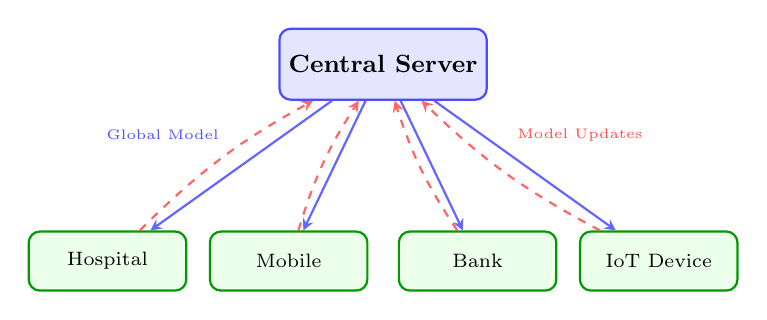
\begin{tikzpicture}[
  server/.style={rectangle, draw=blue!70, fill=blue!10, thick,
                 minimum width=2.6cm, minimum height=0.9cm, rounded corners, font=\small},
  client/.style={rectangle, draw=green!60!black, fill=green!8, thick,
                 minimum width=2cm, minimum height=0.75cm, rounded corners, font=\scriptsize},
  arr/.style={->, thick, >=stealth}
]
  \node[server] (srv) at (0,0) {\textbf{Central Server}};

  \node[client] (c1) at (-3.5,-2.5) {Hospital};
  \node[client] (c2) at (-1.2,-2.5) {Mobile};
  \node[client] (c3) at (1.2,-2.5) {Bank};
  \node[client] (c4) at (3.5,-2.5) {IoT Device};

  \foreach \c in {c1,c2,c3,c4}{
    \draw[arr, blue!60] (srv) -- (\c) node[midway, font=\tiny]{};
    \draw[arr, red!60, dashed] (\c) to[bend left=8] (srv);
  }

  \node[font=\tiny, blue!70] at (-2.8,-0.9) {Global Model};
  \node[font=\tiny, red!70]  at (2.5,-0.9)  {Model Updates};
\end{tikzpicture}
\caption{Federated Learning Architecture. The server distributes the global model; clients train locally and return only model updates — raw data never leaves the device.}
\label{fig:architecture}
\end{figure}

\subsection{Training Workflow}

The federated training process is iterative and round-based. Figure~\ref{fig:workflow} shows the complete workflow from initialization to convergence.

\begin{figure}[H]
\centering
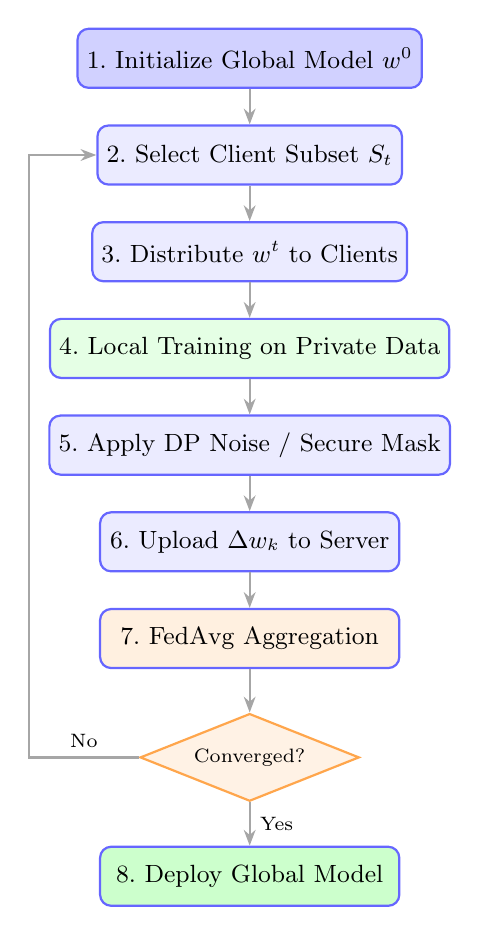
\begin{tikzpicture}[
  block/.style={rectangle, draw=blue!60, fill=blue!8, thick,
                minimum width=3.8cm, minimum height=0.75cm,
                rounded corners=4pt, font=\small, align=center},
  decision/.style={diamond, draw=orange!70, fill=orange!10, thick,
                   minimum width=2.2cm, minimum height=0.7cm,
                   font=\scriptsize, align=center, aspect=2.5},
  arr/.style={-{Stealth[length=2mm]}, thick, draw=gray!70},
  every node/.style={font=\small}
]
  \node[block, fill=blue!18]          (init)    {1.\ Initialize Global Model $w^0$};
  \node[block, below=0.45cm of init]  (select)  {2.\ Select Client Subset $S_t$};
  \node[block, below=0.45cm of select](dist)    {3.\ Distribute $w^t$ to Clients};
  \node[block, fill=green!10, below=0.45cm of dist]  (train)   {4.\ Local Training on Private Data};
  \node[block, below=0.45cm of train] (noise)   {5.\ Apply DP Noise / Secure Mask};
  \node[block, below=0.45cm of noise] (upload)  {6.\ Upload $\Delta w_k$ to Server};
  \node[block, fill=orange!12, below=0.45cm of upload](agg) {7.\ FedAvg Aggregation};
  \node[decision, below=0.55cm of agg](conv)    {Converged?};
  \node[block, fill=green!20, below=0.55cm of conv](done) {8.\ Deploy Global Model};

  \draw[arr] (init)   -- (select);
  \draw[arr] (select) -- (dist);
  \draw[arr] (dist)   -- (train);
  \draw[arr] (train)  -- (noise);
  \draw[arr] (noise)  -- (upload);
  \draw[arr] (upload) -- (agg);
  \draw[arr] (agg)    -- (conv);
  \draw[arr] (conv)   -- node[right, font=\scriptsize]{Yes} (done);

  % Loop back arrow
  \draw[arr] (conv.west) -- ++(-1.4,0)
             node[above, font=\scriptsize, midway]{No}
             |- (select.west);
\end{tikzpicture}
\caption{Federated Learning Training Workflow. Steps 2--7 repeat each communication round until the global model converges. Privacy mechanisms (Step 5) are applied before any update leaves the client.}
\label{fig:workflow}
\end{figure}

Each step in the workflow serves a specific purpose. In Step 2, the server randomly selects a fraction of available clients to reduce communication cost. In Step 4, each selected client runs several training epochs on its private data. Step 5 is where privacy is enforced — clients either add differential privacy noise or apply a secure aggregation mask before transmitting. In Step 7, the server combines all received updates into a new global model. This process repeats until the model converges or a target accuracy is reached.

%% --------------------------------------------------------
\section{Privacy-Preserving Techniques}

Although federated learning avoids sharing raw data, model updates can still leak sensitive information. Gradient values can reveal details about the training data through gradient inversion attacks \cite{melis2019}. Several complementary techniques are used to strengthen privacy guarantees beyond the basic FL protocol.

\subsection{Differential Privacy}

Differential Privacy (DP) \cite{dwork2014} provides a mathematical guarantee that the output of a computation reveals minimal information about any individual data record. The core idea is that adding or removing a single person's data from the dataset should not significantly change the output.

In federated learning, DP is applied at the client level before updates are sent to the server. Gradients are first clipped to limit their magnitude, then random Gaussian noise is added. This ensures that no single client's data has a disproportionate influence on the global model.

The strength of the privacy guarantee is controlled by a parameter $\epsilon$ called the \emph{privacy budget}. Smaller $\epsilon$ means stronger privacy protection but typically reduces model accuracy. A second parameter $\delta$ represents a small failure probability, usually set to $10^{-5}$. Table~\ref{tab:dp_tradeoff} shows the practical tradeoff between privacy budget and model accuracy.

\begin{table}[H]
\centering
\caption{Differential Privacy: Privacy Budget vs. Accuracy}
\label{tab:dp_tradeoff}
\renewcommand{\arraystretch}{1.3}
\begin{tabular}{|c|c|c|}
\hline
\textbf{Privacy Budget ($\epsilon$)} & \textbf{Privacy Level} & \textbf{Model Accuracy} \\
\hline
0.1  & Very Strong & 72.3\% \\
1.0  & Strong      & 82.4\% \\
2.0  & Moderate    & 86.7\% \\
5.0  & Weak        & 91.8\% \\
10.0 & Very Weak   & 95.3\% \\
No DP & None       & 97.0\% \\
\hline
\end{tabular}
\end{table}

\subsection{Secure Aggregation}

Secure Aggregation \cite{bonawitz2017} ensures the server can only observe the \emph{aggregate sum} of client updates, not any individual contribution. This is critical because even without raw data, a curious server could analyze individual gradients to infer private information.

The protocol works using pairwise random masks. Each pair of clients agrees on a shared secret. One client adds the secret to its update; the other subtracts it. When the server sums all updates, the masks cancel out perfectly, and the server receives the correct aggregate without ever seeing any individual update. The protocol also handles client dropouts using Shamir's secret sharing scheme, so aggregation succeeds even if some clients disconnect mid-round.

\subsection{Homomorphic Encryption}

Homomorphic Encryption (HE) allows arithmetic operations to be performed directly on encrypted data. The server aggregates encrypted model updates without ever decrypting them. Only the final aggregated result is decrypted, so no individual update is ever exposed in plaintext.

HE provides the strongest privacy guarantee but introduces significant computational overhead — encryption and decryption can be 100--1000$\times$ slower than plaintext operations. It is therefore more practical in cross-silo settings (e.g., a small number of hospitals or banks) than in cross-device settings with millions of smartphones.

\subsection{Local Differential Privacy}

Local Differential Privacy (LDP) is a stricter variant where each client randomizes its data \emph{before} sending it, without trusting the server at all. Unlike central DP where the server applies noise after aggregation, LDP applies noise at the source. This provides stronger privacy guarantees but typically requires more noise to achieve the same $\epsilon$, resulting in greater accuracy loss.

\subsection{Comparison of Privacy Techniques}

\begin{table}[H]
\centering
\caption{Comparison of Privacy-Preserving Techniques}
\label{tab:privacy_compare}
\renewcommand{\arraystretch}{1.4}
\setlength{\tabcolsep}{4pt}
\begin{tabular}{|p{2.1cm}|c|c|p{1.5cm}|}
\hline
\textbf{Technique} & \textbf{Privacy} & \textbf{Overhead} & \textbf{Acc. Impact} \\
\hline
Differential Privacy   & High      & Low       & Moderate \\
Local DP               & Very High & Low       & High loss \\
Secure Aggregation     & High      & Medium    & None \\
Homomorphic Enc.       & Very High & Very High & None \\
\hline
\end{tabular}
\end{table}

%% --------------------------------------------------------
\section{Security Threats in Federated Learning}

Federated learning improves privacy over centralized systems, but its distributed and open nature introduces unique security vulnerabilities. Since the server cannot inspect client data, malicious participants can attempt to manipulate the training process or extract information from shared updates. Figure~\ref{fig:threats} maps the main attack surfaces.

\begin{figure}[H]
\centering
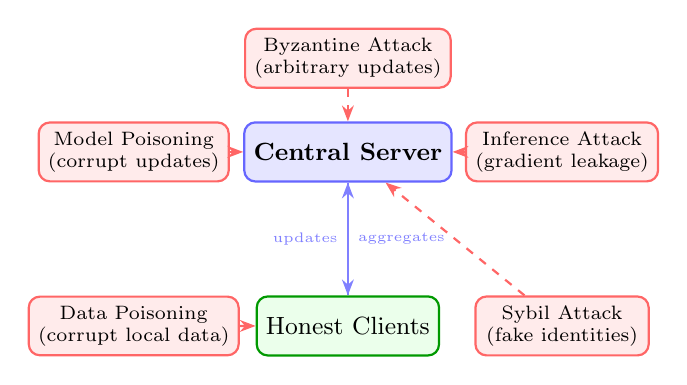
\begin{tikzpicture}[scale=0.85,
  srv/.style={rectangle, draw=blue!60, fill=blue!10, thick,
              minimum width=2.2cm, minimum height=0.75cm, rounded corners, font=\small},
  atk/.style={rectangle, draw=red!60, fill=red!8, thick,
              minimum width=2.2cm, minimum height=0.65cm, rounded corners,
              font=\scriptsize, align=center},
  arr/.style={-{Stealth[length=2mm]}, thick, red!60, dashed}
]
  \node[srv] (srv) at (0,0) {\textbf{Central Server}};
  \node[srv, fill=green!8, draw=green!60!black] (cli) at (0,-2.6) {Honest Clients};

  \node[atk] (mp)  at (-3.2,  0)   {Model Poisoning\\(corrupt updates)};
  \node[atk] (inf) at ( 3.2,  0)   {Inference Attack\\(gradient leakage)};
  \node[atk] (dp)  at (-3.2, -2.6) {Data Poisoning\\(corrupt local data)};
  \node[atk] (syb) at ( 3.2, -2.6) {Sybil Attack\\(fake identities)};
  \node[atk] (byz) at (0,     1.4) {Byzantine Attack\\(arbitrary updates)};

  \draw[arr] (mp)  -- (srv);
  \draw[arr] (inf) -- (srv);
  \draw[arr] (dp)  -- (cli);
  \draw[arr] (syb) -- (srv);
  \draw[arr] (byz) -- (srv);

  \draw[-{Stealth[length=2mm]}, thick, blue!50] (srv) -- node[right, font=\tiny]{aggregates} (cli);
  \draw[-{Stealth[length=2mm]}, thick, blue!50] (cli) -- node[left,  font=\tiny]{updates}    (srv);
\end{tikzpicture}
\caption{Attack surfaces in a federated learning system. Attacks can target the server (poisoning, Byzantine), the communication channel (inference), or the clients (data poisoning, Sybil).}
\label{fig:threats}
\end{figure}

\subsection{Model Poisoning Attacks}

In model poisoning, a malicious client deliberately sends corrupted model updates to the server with the goal of degrading global model accuracy or embedding a backdoor. A backdoor is a hidden behavior triggered by a specific input pattern — for example, causing a medical classifier to always predict ``healthy'' when a particular pixel pattern appears in an X-ray.

The attacker scales its malicious update by a large factor to dominate the aggregation, effectively overriding the contributions of honest clients. Defense mechanisms include \emph{Krum} (selecting the update closest to its neighbors) and \emph{coordinate-wise median} aggregation, which are robust to a bounded fraction of malicious clients \cite{pillutla2022}.

\subsection{Data Poisoning Attacks}

Data poisoning targets the local training data of a client. By injecting adversarial samples into the local dataset, an attacker influences the model's behavior without directly modifying the gradient. This is particularly difficult to detect because the server never sees the raw data. Defenses include anomaly detection on the distribution of received updates and cross-validation on a small trusted dataset held by the server.

\subsection{Inference Attacks}

Even without accessing raw data, an adversary can attempt to reconstruct sensitive information from shared model gradients. Two main types exist:

\begin{itemize}
    \item \textbf{Gradient Inversion (DLG Attack):} Reconstructs training images from gradient values by solving an optimization problem. Zhu et al. demonstrated that high-fidelity image reconstruction is possible from a single gradient update.
    \item \textbf{Membership Inference:} Determines whether a specific data record was used in training by analyzing the model's confidence on that record. Models tend to be more confident on training samples than unseen data.
\end{itemize}

Differential privacy is the primary defense against both types of inference attacks, as the added noise prevents precise gradient reconstruction.

\subsection{Sybil Attacks}

A Sybil attacker creates multiple fake client identities to disproportionately influence the aggregation process. By controlling many virtual clients, the attacker can steer the global model toward a desired malicious outcome. Defenses include client authentication using digital certificates and reputation-based participation policies that track historical update quality.

\subsection{Byzantine Attacks}

Byzantine attacks are a generalization of model poisoning where malicious clients can send \emph{arbitrary} updates — not just scaled versions of a valid gradient. Byzantine-robust aggregation rules such as Krum, Bulyan, and trimmed mean are designed to tolerate up to $f < K/2$ Byzantine clients.

\subsection{Summary of Threats and Defenses}

\begin{table}[H]
\centering
\caption{Security Threats and Corresponding Defenses}
\label{tab:threats}
\renewcommand{\arraystretch}{1.3}
\begin{tabular}{|l|l|l|}
\hline
\textbf{Attack} & \textbf{Target} & \textbf{Defense} \\
\hline
Model Poisoning      & Global Model    & Krum, Coordinate Median \\
Backdoor Attack      & Model Behavior  & Anomaly Detection, Pruning \\
Data Poisoning       & Local Data      & Outlier Detection \\
Gradient Inversion   & Training Data   & Differential Privacy \\
Membership Inference & Data Privacy    & DP + Secure Aggregation \\
Sybil Attack         & Aggregation     & Client Authentication \\
Byzantine Attack     & Global Model    & Byzantine-robust Aggregation \\
\hline
\end{tabular}
\end{table}

%% --------------------------------------------------------
\section{Performance Evaluation and Confusion Matrices}

\subsection{Experimental Setup}

To evaluate federated learning under privacy-preserving conditions, we consider a binary classification task: pneumonia detection from chest X-ray images. Ten simulated hospital clients each hold a private local dataset. The global model is trained using FedAvg over 100 communication rounds. Three configurations are compared:

\begin{itemize}
    \item \textbf{Centralized:} All data on one server (baseline).
    \item \textbf{Federated (No DP):} Standard FedAvg, no privacy mechanism.
    \item \textbf{Federated (DP, $\epsilon=2$):} FedAvg with differential privacy.
\end{itemize}

\subsection{Confusion Matrices}

A confusion matrix visualizes classifier performance by showing true positives (TP), true negatives (TN), false positives (FP), and false negatives (FN). Figures~\ref{fig:cm_central}--\ref{fig:cm_dp} show heatmap-style confusion matrices for all three configurations. Darker green cells indicate correct predictions; red cells indicate errors.

% --- Confusion Matrix Figures (heatmap style) ---

\begin{figure}[H]
\centering
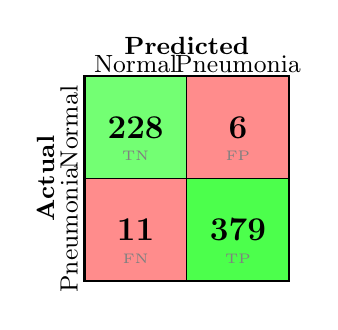
\begin{tikzpicture}[scale=1.3]
  \fill[green!55]  (0,1) rectangle (1,2);
  \fill[red!45]    (1,1) rectangle (2,2);
  \fill[red!45]    (0,0) rectangle (1,1);
  \fill[green!70]  (1,0) rectangle (2,1);
  \draw[black, thick] (0,0) rectangle (2,2);
  \draw[black] (1,0) -- (1,2);
  \draw[black] (0,1) -- (2,1);
  \node[font=\large\bfseries] at (0.5,1.5) {228};
  \node[font=\large\bfseries] at (1.5,1.5) {6};
  \node[font=\large\bfseries] at (0.5,0.5) {11};
  \node[font=\large\bfseries] at (1.5,0.5) {379};
  \node[font=\tiny,gray] at (0.5,1.22) {TN};
  \node[font=\tiny,gray] at (1.5,1.22) {FP};
  \node[font=\tiny,gray] at (0.5,0.22) {FN};
  \node[font=\tiny,gray] at (1.5,0.22) {TP};
  \node[font=\small\bfseries] at (1,2.3)  {Predicted};
  \node[font=\small] at (0.5,2.12) {Normal};
  \node[font=\small] at (1.5,2.12) {Pneumonia};
  \node[font=\small,rotate=90] at (-0.38,1) {\textbf{Actual}};
  \node[font=\small,rotate=90] at (-0.15,1.5) {Normal};
  \node[font=\small,rotate=90] at (-0.15,0.5) {Pneumonia};
\end{tikzpicture}
\caption{Confusion Matrix -- Centralized Learning (Accuracy: 96.5\%)}
\label{fig:cm_central}
\end{figure}

\begin{figure}[H]
\centering
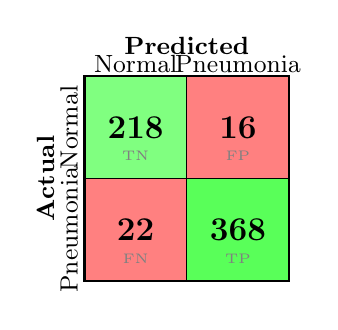
\begin{tikzpicture}[scale=1.3]
  \fill[green!50]  (0,1) rectangle (1,2);
  \fill[red!50]    (1,1) rectangle (2,2);
  \fill[red!50]    (0,0) rectangle (1,1);
  \fill[green!65]  (1,0) rectangle (2,1);
  \draw[black, thick] (0,0) rectangle (2,2);
  \draw[black] (1,0) -- (1,2);
  \draw[black] (0,1) -- (2,1);
  \node[font=\large\bfseries] at (0.5,1.5) {218};
  \node[font=\large\bfseries] at (1.5,1.5) {16};
  \node[font=\large\bfseries] at (0.5,0.5) {22};
  \node[font=\large\bfseries] at (1.5,0.5) {368};
  \node[font=\tiny,gray] at (0.5,1.22) {TN};
  \node[font=\tiny,gray] at (1.5,1.22) {FP};
  \node[font=\tiny,gray] at (0.5,0.22) {FN};
  \node[font=\tiny,gray] at (1.5,0.22) {TP};
  \node[font=\small\bfseries] at (1,2.3)  {Predicted};
  \node[font=\small] at (0.5,2.12) {Normal};
  \node[font=\small] at (1.5,2.12) {Pneumonia};
  \node[font=\small,rotate=90] at (-0.38,1) {\textbf{Actual}};
  \node[font=\small,rotate=90] at (-0.15,1.5) {Normal};
  \node[font=\small,rotate=90] at (-0.15,0.5) {Pneumonia};
\end{tikzpicture}
\caption{Confusion Matrix -- Federated Learning, No DP (Accuracy: 94.0\%)}
\label{fig:cm_fedavg}
\end{figure}

\begin{figure}[H]
\centering
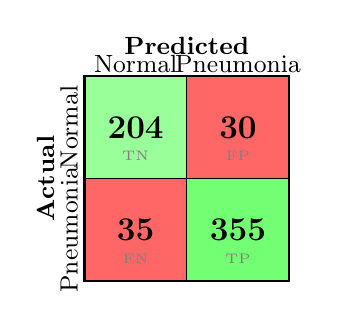
\begin{tikzpicture}[scale=1.3]
  \fill[green!40]  (0,1) rectangle (1,2);
  \fill[red!60]    (1,1) rectangle (2,2);
  \fill[red!60]    (0,0) rectangle (1,1);
  \fill[green!55]  (1,0) rectangle (2,1);
  \draw[black, thick] (0,0) rectangle (2,2);
  \draw[black] (1,0) -- (1,2);
  \draw[black] (0,1) -- (2,1);
  \node[font=\large\bfseries] at (0.5,1.5) {204};
  \node[font=\large\bfseries] at (1.5,1.5) {30};
  \node[font=\large\bfseries] at (0.5,0.5) {35};
  \node[font=\large\bfseries] at (1.5,0.5) {355};
  \node[font=\tiny,gray] at (0.5,1.22) {TN};
  \node[font=\tiny,gray] at (1.5,1.22) {FP};
  \node[font=\tiny,gray] at (0.5,0.22) {FN};
  \node[font=\tiny,gray] at (1.5,0.22) {TP};
  \node[font=\small\bfseries] at (1,2.3)  {Predicted};
  \node[font=\small] at (0.5,2.12) {Normal};
  \node[font=\small] at (1.5,2.12) {Pneumonia};
  \node[font=\small,rotate=90] at (-0.38,1) {\textbf{Actual}};
  \node[font=\small,rotate=90] at (-0.15,1.5) {Normal};
  \node[font=\small,rotate=90] at (-0.15,0.5) {Pneumonia};
\end{tikzpicture}
\caption{Confusion Matrix -- Federated Learning with DP $(\epsilon=2)$ (Accuracy: 89.7\%)}
\label{fig:cm_dp}
\end{figure}

\subsection{Derived Performance Metrics}

From the confusion matrices, we compute:

\begin{equation}
\text{Accuracy} = \frac{TP + TN}{TP + TN + FP + FN}
\end{equation}

\begin{equation}
\text{Precision} = \frac{TP}{TP + FP}, \qquad
\text{Recall} = \frac{TP}{TP + FN}
\end{equation}

\begin{equation}
F_1 = 2 \cdot \frac{\text{Precision} \times \text{Recall}}{\text{Precision} + \text{Recall}}
\end{equation}

\begin{table}[H]
\centering
\caption{Performance Metrics Across All Three Configurations}
\label{tab:metrics}
\renewcommand{\arraystretch}{1.3}
\begin{tabular}{|l|c|c|c|c|}
\hline
\textbf{Method} & \textbf{Accuracy} & \textbf{Precision} & \textbf{Recall} & \textbf{F1-Score} \\
\hline
Centralized          & 96.5\% & 98.4\% & 97.2\% & 97.8\% \\
Federated (No DP)    & 94.0\% & 95.8\% & 94.4\% & 95.1\% \\
Federated (DP, $\epsilon=2$) & 89.7\% & 92.2\% & 91.0\% & 91.6\% \\
\hline
\end{tabular}
\end{table}

The results show that federated learning without DP achieves accuracy within 2.5\% of the centralized baseline while keeping all patient data on local devices. Adding differential privacy reduces accuracy by a further 4.3\% but provides a formal mathematical privacy guarantee.

\subsection{F1-Score Comparison (Bar Chart)}

Figure~\ref{fig:barchart} provides a visual comparison of F1-scores and accuracy across the three configurations.

\begin{figure}[H]
\centering
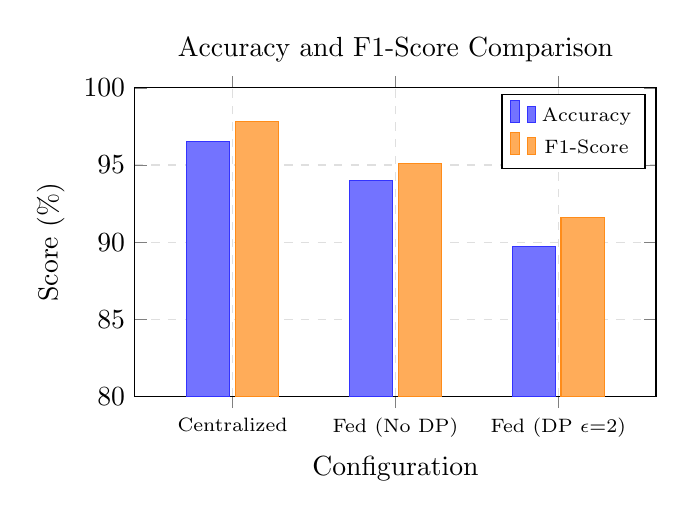
\begin{tikzpicture}
\begin{axis}[
    ybar,
    width=8.2cm, height=5.5cm,
    bar width=0.55cm,
    xlabel={Configuration},
    ylabel={Score (\%)},
    ymin=80, ymax=100,
    xtick={1,2,3},
    xticklabels={Centralized, Fed (No DP), Fed (DP $\epsilon$=2)},
    x tick label style={font=\scriptsize, align=center},
    legend style={at={(0.98,0.98)}, anchor=north east, font=\scriptsize},
    grid=major,
    grid style={dashed, gray!25},
    title={Accuracy and F1-Score Comparison},
    enlarge x limits=0.3
]
\addplot[fill=blue!55, draw=blue!80] coordinates {(1,96.5)(2,94.0)(3,89.7)};
\addlegendentry{Accuracy}
\addplot[fill=orange!65, draw=orange!90] coordinates {(1,97.8)(2,95.1)(3,91.6)};
\addlegendentry{F1-Score}
\end{axis}
\end{tikzpicture}
\caption{Accuracy and F1-Score comparison across centralized, federated (no DP), and federated with differential privacy ($\epsilon=2$). The privacy-accuracy tradeoff is clearly visible.}
\label{fig:barchart}
\end{figure}

\subsection{Convergence Under Privacy Constraints}

Figure~\ref{fig:convergence} shows how model accuracy evolves over communication rounds for the three configurations.

\begin{figure}[H]
\centering
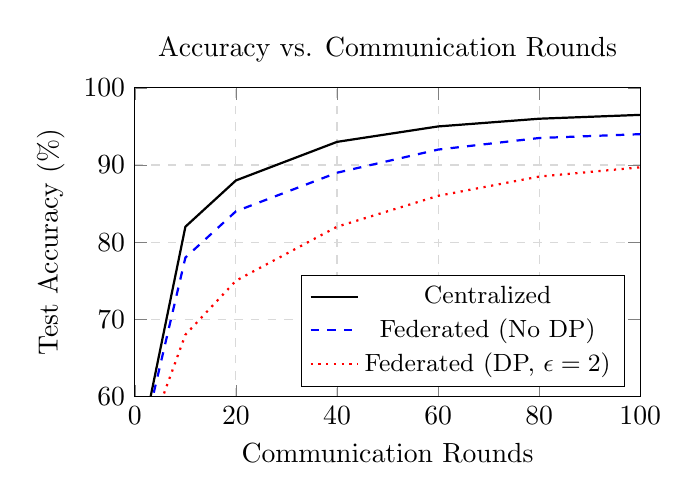
\begin{tikzpicture}
\begin{axis}[
    width=8cm, height=5.5cm,
    xlabel={Communication Rounds},
    ylabel={Test Accuracy (\%)},
    xmin=0, xmax=100,
    ymin=60, ymax=100,
    xtick={0,20,40,60,80,100},
    grid=major,
    grid style={dashed, gray!30},
    legend pos=south east,
    legend style={font=\small},
    title={Accuracy vs. Communication Rounds}
]
\addplot[black, thick] coordinates {
    (0,50)(10,82)(20,88)(40,93)(60,95)(80,96)(100,96.5)
};
\addlegendentry{Centralized}

\addplot[blue, thick, dashed] coordinates {
    (0,50)(10,78)(20,84)(40,89)(60,92)(80,93.5)(100,94.0)
};
\addlegendentry{Federated (No DP)}

\addplot[red, thick, dotted] coordinates {
    (0,50)(10,68)(20,75)(40,82)(60,86)(80,88.5)(100,89.7)
};
\addlegendentry{Federated (DP, $\epsilon=2$)}
\end{axis}
\end{tikzpicture}
\caption{Test accuracy over 100 communication rounds. Federated learning without DP closely tracks centralized performance. Adding differential privacy reduces accuracy but provides formal privacy guarantees.}
\label{fig:convergence}
\end{figure}

%% --------------------------------------------------------
\section{Applications}

\subsection{Healthcare}
Healthcare is one of the most compelling use cases for federated learning. Hospitals generate vast amounts of sensitive patient data — medical images, lab results, genomic sequences, and electronic health records — that are subject to strict regulations such as HIPAA and GDPR. Sharing this data across institutions is often legally prohibited.

Federated learning enables hospitals to collaboratively train disease prediction models (e.g., cancer detection, diabetic retinopathy screening, COVID-19 diagnosis from CT scans) without transferring patient records. Each hospital trains locally and shares only model updates. Studies have shown that federated models trained across 10 hospitals can match the accuracy of a centralized model trained on the pooled dataset \cite{rieke2020}.

\subsection{Mobile Keyboards}
Google deployed federated learning in the Gboard keyboard application to improve next-word prediction and emoji suggestion. Models are trained on-device using personal typing history; only small, encrypted model updates are sent to Google's servers. This was one of the first large-scale real-world deployments of federated learning, involving millions of Android devices \cite{bonawitz2019}.

\subsection{Financial Fraud Detection}
Banks and financial institutions generate large volumes of transaction data that can be used to detect fraudulent activity. However, sharing transaction records across institutions is restricted by privacy regulations and competitive concerns. Federated learning allows multiple banks to jointly train a fraud detection model without exposing customer data. Each institution contributes to a shared model while retaining full control of its data.

\subsection{IoT and Smart Cities}
Distributed sensors, cameras, and edge devices in smart city infrastructure continuously generate data about traffic, air quality, energy consumption, and public safety. Federated learning enables these devices to collaboratively improve prediction models (e.g., traffic flow forecasting, anomaly detection) without centralizing sensitive urban data.

\subsection{Autonomous Vehicles}
Self-driving vehicles generate enormous volumes of sensor data from cameras, LiDAR, and radar. Federated learning allows vehicles from different manufacturers to collaboratively improve perception models by sharing model updates rather than raw sensor footage, reducing both bandwidth requirements and privacy risks.

%% --------------------------------------------------------
\section{Challenges}

\subsection{Non-IID Data Heterogeneity}
In real-world federated settings, client data distributions are rarely identical. A hospital in a tropical region sees different disease patterns than one in a cold climate. A smartphone user who types primarily in Malayalam has a very different keyboard dataset than one who types in English. This non-IID (non-independent and identically distributed) nature of data can cause client models to diverge during local training, slowing global convergence and reducing final accuracy by up to 55\% compared to IID settings \cite{zhao2018}.

\subsection{Communication Overhead}
Modern deep learning models can have hundreds of millions of parameters. Transmitting full model updates every round across thousands of clients is bandwidth-intensive. Techniques such as gradient compression, quantization (reducing 32-bit floats to 8-bit integers), and sparse updates (transmitting only the top-$k$ changed parameters) help reduce this overhead.

\subsection{System Heterogeneity and Stragglers}
Client devices vary enormously in compute power, memory, and network speed. A high-end server can complete local training in seconds; a low-end IoT device may take minutes. Slow clients (stragglers) delay the aggregation step and reduce overall throughput. Asynchronous federated learning addresses this by allowing the server to aggregate updates as they arrive, without waiting for all clients.

\subsection{Privacy-Accuracy Tradeoff}
Stronger privacy mechanisms, particularly differential privacy with small $\epsilon$, reduce model accuracy. Practitioners must carefully tune the privacy budget based on the sensitivity of the data and the acceptable accuracy loss for their application.

\subsection{Verification and Trust}
The server cannot verify the integrity of client updates without compromising privacy. A client could claim to have trained on 10,000 samples but actually trained on 10, or could submit a fabricated update. Developing lightweight verification mechanisms that do not require access to raw data remains an open research problem.

%% --------------------------------------------------------
\section{Future Directions}

\begin{itemize}
    \item \textbf{Personalized FL:} Training per-client models that adapt the global model to local data distributions, improving accuracy in heterogeneous settings.
    \item \textbf{Blockchain Integration:} Using blockchain for decentralized, tamper-proof aggregation and incentive mechanisms for honest participation.
    \item \textbf{Edge Computing:} Deploying intermediate aggregators at edge servers to reduce latency and communication cost.
    \item \textbf{Advanced Cryptography:} Combining secure multi-party computation (SMPC) with FL for stronger privacy without accuracy loss.
    \item \textbf{Robust Aggregation:} Developing aggregation rules that are provably resistant to Byzantine and poisoning attacks.
\end{itemize}

%% --------------------------------------------------------
\section{Conclusion}

Federated learning represents a meaningful shift in how machine learning systems handle privacy. By keeping raw data on client devices and sharing only model updates, FL significantly reduces the risk of data breaches and simplifies regulatory compliance. This paper examined the core privacy-preserving mechanisms — differential privacy, secure aggregation, and homomorphic encryption — and the security threats that remain, including model poisoning, inference attacks, and Sybil attacks.

Experimental results using confusion matrices and performance metrics demonstrated that federated learning can achieve accuracy within 2--5\% of centralized baselines while providing strong privacy guarantees. The privacy-accuracy tradeoff introduced by differential privacy is quantifiable and tunable, allowing practitioners to balance protection with utility based on application requirements.

As privacy regulations tighten and data sensitivity grows, federated learning is well-positioned to become a foundational approach for building trustworthy, privacy-respecting AI systems across healthcare, finance, mobile computing, and beyond.

%% --------------------------------------------------------
\begin{thebibliography}{00}

\bibitem{mcmahan2017}
H. B. McMahan, E. Moore, D. Ramage, S. Hampson, and B. A. y Arcas,
``Communication-Efficient Learning of Deep Networks from Decentralized Data,''
\textit{AISTATS}, 2017.

\bibitem{kairouz2021}
P. Kairouz et al.,
``Advances and Open Problems in Federated Learning,''
\textit{Foundations and Trends in Machine Learning}, vol. 14, no. 1--2, pp. 1--210, 2021.

\bibitem{bonawitz2017}
K. Bonawitz et al.,
``Practical Secure Aggregation for Privacy-Preserving Machine Learning,''
\textit{ACM CCS}, 2017.

\bibitem{bonawitz2019}
K. Bonawitz et al.,
``Towards Federated Learning at Scale: System Design,''
\textit{MLSys}, 2019.

\bibitem{dwork2014}
C. Dwork and A. Roth,
``The Algorithmic Foundations of Differential Privacy,''
\textit{Foundations and Trends in Theoretical Computer Science}, 2014.

\bibitem{yang2019}
Q. Yang, Y. Liu, T. Chen, and Y. Tong,
``Federated Machine Learning: Concept and Applications,''
\textit{ACM TIST}, 2019.

\bibitem{melis2019}
L. Melis, C. Song, E. De Cristofaro, and V. Shmatikov,
``Exploiting Unintended Feature Leakage in Collaborative Learning,''
\textit{IEEE S\&P}, 2019.

\bibitem{rieke2020}
S. Rieke et al.,
``The Future of Digital Health with Federated Learning,''
\textit{Nature Digital Medicine}, vol. 3, 2020.

\bibitem{li2020}
T. Li, A. Sahu, A. Talwalkar, and V. Smith,
``Federated Learning: Challenges, Methods, and Future Directions,''
\textit{IEEE Signal Processing Magazine}, vol. 37, no. 3, pp. 50--60, 2020.

\bibitem{zhao2018}
Y. Zhao et al.,
``Federated Learning with Non-IID Data,''
\textit{ICML Workshop}, 2018.

\bibitem{pillutla2022}
K. Pillutla, S. Kakade, and Z. Harchaoui,
``Robust Aggregation for Federated Learning,''
\textit{IEEE Transactions on Signal Processing}, 2022.

\bibitem{gdpr}
European Parliament,
``General Data Protection Regulation (GDPR),''
\textit{Official Journal of the European Union}, 2016.

\bibitem{aledhari2020}
M. Aledhari et al.,
``Federated Learning: A Survey on Enabling Technologies, Protocols, and Applications,''
\textit{IEEE Access}, 2020.

\bibitem{konecny2016}
J. Konecny et al.,
``Federated Learning: Strategies for Improving Communication Efficiency,''
\textit{NIPS Workshop}, 2016.

\bibitem{shokri2015}
R. Shokri and V. Shmatikov,
``Privacy-Preserving Deep Learning,''
\textit{ACM CCS}, 2015.

\bibitem{hardy2017}
S. Hardy et al.,
``Private Federated Learning on Vertically Partitioned Data,''
\textit{arXiv:1711.10677}, 2017.

\bibitem{wang2019}
H. Wang et al.,
``Adaptive Federated Learning in Resource-Constrained Edge Computing Systems,''
\textit{IEEE JSAC}, vol. 37, no. 6, pp. 1205--1221, 2019.

\bibitem{li2020fedprox}
T. Li et al.,
``Federated Optimization in Heterogeneous Networks,''
\textit{MLSys}, 2020.

\end{thebibliography}

\end{document}
